% Headers
\documentclass[12pt]{article}
\usepackage{graphics}
\usepackage{verbatim}
\usepackage{amsmath}
\usepackage{enumerate}
\usepackage{graphicx}
\usepackage{listings}
\usepackage{mathtools}
\usepackage{fancyvrb}
\usepackage{enumitem}

\title{\textbf{CMPS 111 Operating Systems\\ Winter 2018, Homework \#4}}
\date{}
\author{Aaron Steele, atsteele@ucsc.edu}

\begin{document}
	
	\maketitle
	
	\section*{Question 1}
	An Access Control List and a Capability List are two different ways of representing data from an Access Matrix. An ACL is the columns of the matrix, with the file/resource as the key of the list, and the users' permission levels being the values. 
	
	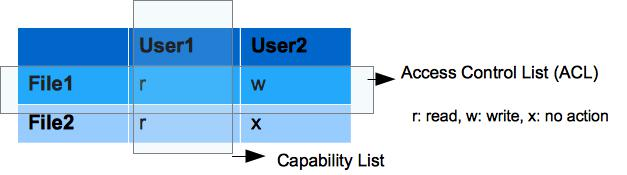
\includegraphics[width=\columnwidth]{access-matrix}
	
	A Capability List is the rows of the Access Matrix, taking the user as the key and the file/resource permission levels as the values. 
	\begin{enumerate}[label=\alph*]
		\item An ACL. Just loop across the list at index of your resource, and set everything to Read.
		\item An ACL. Same as (a), loop over the list at the index of the resource, and remove the Write access for everyone.
		\item A Capability List. Simply go to the Users you want to give access to, then search the list to find the file, and set that value to Write. Do this for all three users.
		\item A Capability List. For the same reasons as (c). Find the users and then search the list to revoke the specific accesses.
	\end{enumerate}
	
	
	\section*{Question 2}
	\subsection*{A}
	The processor that has a single cache where it stores the data and executable code is more vulnerable to a buffer overflow attack. This is simply because a buffer cannot overflow into a location that is not next to it. So, having the buffer where program data is stored be separate from where the code is prevents anything that is entered into a program as data is not able to be executed by the operating system.
	
	\subsection*{B}
	The first way an OS can protect itself against buffer overflow attacks is to separate the data and executable code buffers in software. Having them separate in software and hardware is best, but the hardware portion requires a change in chip design. Separating them in software makes it much harder to overflow from the data buffer into the executable buffer, if not impossible. 
	
	A second way for an OS to protect itself from a buffer overflow attack is to not allow functions that are overflow-able. The example in class was gets(). The operating system could disallow known exploitable functions from even running, which would cut down on exploits from programmers that aren't aware of them drastically. But this comes with the tradeoff of not being backwards-compatible, which is a big deal and would very likely break old programs that have no support anymore. 
	
	
	\section*{Question 3}
	Which hole is taken for successive segment requests of\\
	12 MB, 10 MB, 9 MB?
	
	Note: The memory is from left to right, and a 0 in the Process line means nothing was placed there.
			
	\subsection*{(A)}
	First fit - Go from left to right and place the process in the first location that has enough space for it to fit.
	
	\begin{tabular}[c]{| l | l | l | l | l | l | l | l | l |}
		\hline
		Holes & 10MB & 4MB & 20MB & 18MB & 7MB & 9MB & 12MB & 15MB \\
		\hline
		Process & 10MB & 0 & 12MB & 9MB & 0 & 0 & 0 & 0 \\
		\hline
	\end{tabular}
	
	\subsection*{(B)}
	Best fit - Scan the list and place the process in the hole that has the closest amount of space to the process' requirement
	
	\begin{tabular}[c]{| l | l | l | l | l | l | l | l | l |}
		\hline
		Holes & 10MB & 4MB & 20MB & 18MB & 7MB & 9MB & 12MB & 15MB \\
		\hline
		Process & 10MB & 0 & 0 & 0 & 0 & 9MB & 12MB & 0 \\
		\hline
	\end{tabular}
	
	\subsection*{(C)}	
	Worst fit - Scan the list and place the process in the hole that has the largest amount of memory
	
	\begin{tabular}[c]{| l | l | l | l | l | l | l | l | l |}
		\hline
		Holes & 10MB & 4MB & 20MB & 18MB & 7MB & 9MB & 12MB & 15MB \\
		\hline
		Process & 0 & 0 & 12MB & 10MB & 0 & 0 & 0 & 9MB \\
		\hline
	\end{tabular}
	
	\subsection*{(D)}
	Next fit - Similar to first fit, but after the first run, continue scanning for the next hole that fits from the location of the last insertion.
	
	\begin{tabular}[c]{| l | l | l | l | l | l | l | l | l |}
		\hline
		Holes & 10MB & 4MB & 20MB & 18MB & 7MB & 9MB & 12MB & 15MB \\
		\hline
		Process & 0 & 0 & 12MB & 10MB & 0 & 9MB & 0 & 0 \\
		\hline
	\end{tabular}
	
	\section*{Question 4}
	A computer with a 32-bit processor uses a two-level page lookup mechanism
	consisting of page tables and a page table directory. Virtual Addresses consist of a 9-bit page table
	directory field, an 11-bit page table field, and an offset. How large are the pages and how many are
	there in the address space?
	
	$$ 32 - \text{directory} - \text{pageTable} - \text{offset} = 32 - 9 - 11 = 12\text{-bit offset}$$
	$$ 2^{12} = 4,096 \text{bits} = 4KB \text{ pages} $$
	$$ 32 - 12 = 20 \text{bits for virtual pages. So, } 2^{20} \text{ pages} $$
	
	\section*{Question 5}	
	\subsection*{(A)}
	\begin{figure}
		\centering
		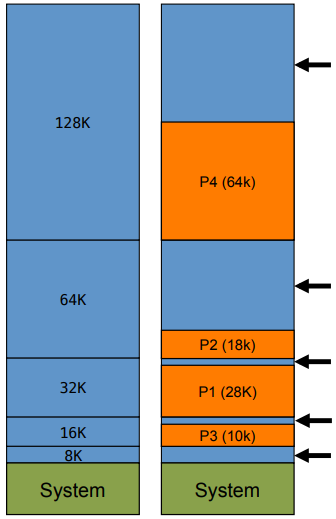
\includegraphics[width=0.3\columnwidth]{internal-fragmentation}
		\caption{Internal Fragmentation}
		\label{int-frag}
	\end{figure}
	
	\begin{figure}
		\centering
		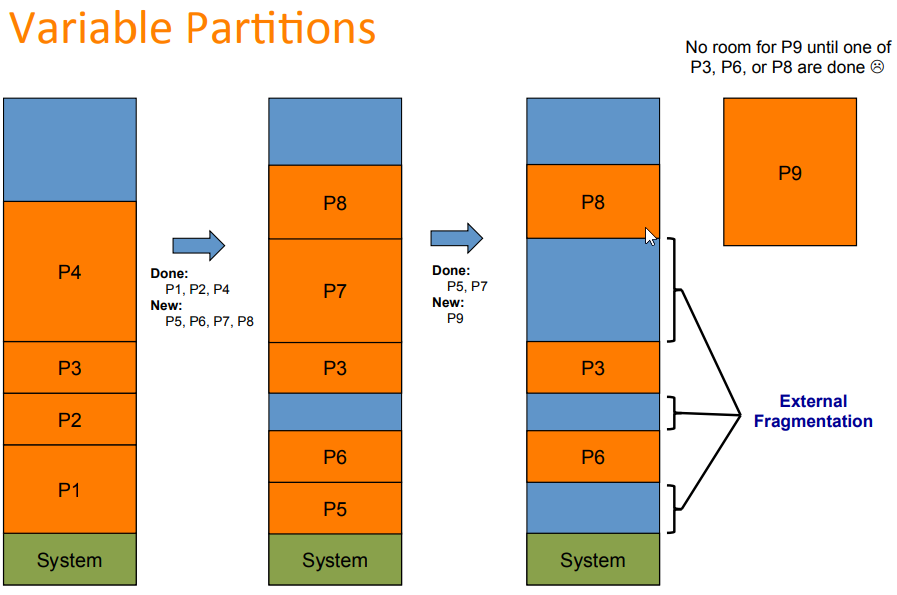
\includegraphics[width=0.8\columnwidth]{external-fragmentation}
		\caption{External Fragmentation}
		\label{ext-frag}
	\end{figure}

	\begin{itemize}
		\item Internal fragmentation - This can only happen with fixed memory partitions. There is a lot of wasted space in memory when programs that are considerably smaller than the smallest partition they can fit into are ran. In the example graphic (Figure \ref{int-frag}), P2 is run after P1, and so P2 must be put into the partition with 64k memory, even though it only uses 18k. This creates a very large amount of empty space that is unusable until P2 is finished its execution.
		
		\item External fragmentation - Can only happen when the partitions are variable. As processes finish running the locations they were put in memory are freed up, but if other processes are still running higher in the memory block, this can create a problem. Consider Figure \ref{ext-frag}, where P9 cannot be executed until there is enough space to fit it in, even though there is enough raw memory available to run it, it's arranged in such a way that P8, P6, or P3 must finish before P9 can have enough space to execute.
	\end{itemize}

	\subsection*{(B)}
	Paging is the modern solution to the problem of how to allocate memory to programs. We face issues of fragmentation in statically and variably partitioned memory, so the solution that we have come up with is to create a virtual memory space for each program, and then the OS and hardware coordinate to link the virtual addresses to the physical memory. See Figure \ref{paging-overview}.
	
	Each program has a much larger virtual memory than physical, this allows the program to view the memory as contiguous and easily accessible. 
	
	Instead of storing each mapping of virtual to physical in an array that would naturally have large amounts of unused space, we create a hierarchical data structure of page tables and a page table directory. Then when a process need to store data into the page table directory, if the specific page table is not yet initialized, we initialize it, which saves on in-RAM space.
	
	
	\begin{figure}
		\centering
		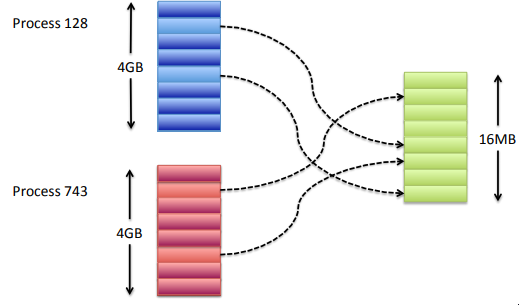
\includegraphics[width=\columnwidth]{paging-overview}
		\caption{Paging Overview}
		\label{paging-overview}
	\end{figure}
	
	
	\subsection*{(C)}
	Compaction is when in variably partitioned memory, all the processes are told to pause while the operating system rearranges the processes memory locations to all be contiguous near the bottom of the memory. This is a memory defragmentation technique. A major problem with this technique is the pause signal that must to out to all processes. On a modern machine, this could happen every few seconds, or even faster, depending on what the computer was doing. This would create a large slowdown, especially compared to paging.
	
	Paging has no point where all the processes are told to pause to let the OS reorganize the memory, which means it is faster. Considering speed is of the utmost importance to an operating system, it is no surprise why this method won out over compacting, even though it is much more complicated, requiring extra hardware components and much more software code.
	
\end{document}